\documentclass[xcolor=dvipsnames,10pt]{beamer}
%\usetheme{Berkeley}
\usetheme{Warsaw} 
\usecolortheme{default}

\usepackage[latin1]{inputenc}
\usepackage[brazil]{babel}  
\usepackage{pstricks}
\usepackage{amssymb}

\begin{document}
%-------------------------------------------------------------------------------------------------
%-------------------------------------------------------------------------------------------------
\author{Tassiano Neuhaus}
\institute[]{PPGEE - UFRGS}
%-------------------------------------------------------------------------------------------------
%-------------------------------------------------------------------------------------------------
%\subject{} \AtBeginSubsection[]
%{
%	\begin{frame}<beamer>
%		\frametitle{Plan wyk�adu}
%		\tableofcontents[currentsection,currentsubsection]
%	\end{frame}
%}

\title[PPGEE - UFRGS]{Projeto de controladores n�o lineares utilizando refer�ncia virtual}
\subtitle{Disserta��o de mestrado}

\date{Setembro de 2012}

\begin{frame}\titlepage
\end{frame} 

\begin{frame}
\frametitle{Agenda}\tableofcontents
\end{frame} 

% Motiva��o
% - porque usar identifica��o de sistemas n�o lineares

% Introdu��o a identifica��o de sistemas
%  - conceitos b�sicos e defini��es de variaveis

% Modelos n�o lineares
% - Modelos racionais NARMAX

% Projeto de controladores
% - Conceitos b�sicosde identifica��o baseados em dados

% Utiliza��o Refer�ncia virtual 
% N�o linearidades est�ticas
% - exemplos - resultdos obtidos
% n�o linearidades dinamicas (modelos racionais)
% exemplos  - resultados obtidos
%
% Conclus�es
%-------------------------------------------------------------------------------------------------
%-------------------------------------------------------------------------------------------------

%-------------------------------------------------------------------------------------------------
\section{Objetivo e Motiva��o}
\subsection{ssss}
%-------------------------------------------------------------------------------------------------
\begin{frame}
\frametitle{Objetivo / Motiva��o}

\begin{block}{Objetivo}
Apresentar um estudo sobre projeto de controladores n�o lineares utilizando conceito de identifica��o de
sistemas e de refer�ncia virtual para obten��o dos dados necess�rios.
\end{block}

\begin{block}{Motiva��o}
\begin{itemize}
	\item Controladores n�o lineares s�o pouco explorados
	\item Para alguns tipos de sistemas, controladores n�o lineares conseguem ser mais perform�ticos
\end{itemize}
\end{block}

\end{frame}


%-------------------------------------------------------------------------------------------------
\section{Defini��es} 
%-------------------------------------------------------------------------------------------------
\begin{frame}
\frametitle{Defini��es}

\begin{block}{Foco em sistemas SISO}
Sistemas {\it{Single input single output}} (SISO) discretos:
\begin{equation}
y(t)=G_0(z)u(t)+H_0(z)e(t)
\nonumber
\end{equation}
onde $G_0(z)$ � a representa��o da planta real do sistema, $H_0(z)$ � a representa��o do filtro que atua sobre o ru�do
branco $e(t)$. $y(t)$ � a sa�da e $u(t)$ � a entrada do sistema.

\end{block}
\end{frame}

%-------------------------------------------------------------------------------------------------
\subsection{Identifica��o de sistemas} 
%-------------------------------------------------------------------------------------------------

\begin{frame}
\frametitle{Defini��es}
\framesubtitle{Identifica��o de sistemas}
Identifica��o de sistemas cont�m tr�s componentes principais:

\begin{itemize}
	\item O sistema real a ser identificado $\mathcal{S}$
 	\begin{equation}
		\mathcal{S}:\;\; y(t)=G_0(z)u(t)+H_0(z)e(t)
		\label{eq:si_intro_true_system}
	\end{equation}

	\item A classe de modelos a ser utilizada na identifica��o $\mathcal{M}$
	\begin{equation}
		\mathcal{M}: \;\;\left \{ G(z, \theta), H(z, \theta) | \theta \in D_{\mathcal{M}} \right \}
		\label{eq:si_intro_model}
	\end{equation}

\end{itemize}
\end{frame}
%-------------------------------------------------------------------------------------------------
%-------------------------------------------------------------------------------------------------

\begin{frame}
\frametitle{Defini��es}
\framesubtitle{Identifica��o de sistemas}

\begin{itemize}
	\item Algum crit�rio para elencar qual modelo dentro da classe de modelos melhor
	consegue representar o sistema $\mathcal{S}$ nas propriedades escolhidas.
	\begin{block}{Neste trabalho optou-se por:}
	\begin{equation}
		V(\theta)=\frac{1}{N}\sum_{t=1}^{N}\frac{1}{2} \varepsilon ^2(t, \theta)
		\label{eq:si_obj_etim_lsm_v}
	\end{equation}
	\end{block}
	onde $\varepsilon (t,\theta)$ � o erro de predi��o e pode ser definido como:
	
	\begin{equation}
		\varepsilon (t,\theta)=H^{-1}(z, \theta)\left \{ y(t)-G(z, \theta)u(t) \right \}
	\nonumber
	\end{equation}
\end{itemize}
\end{frame}

%-------------------------------------------------------------------------------------------------
\subsection{Propriedades estat�sticas das estimativas} 
%-------------------------------------------------------------------------------------------------
\begin{frame}
\frametitle{Defini��es}
\framesubtitle{Propriedades estat�sticas das estimativas}

\begin{itemize}
  \item $\theta_0$: conjunto de par�metros que faz com que:
  
  \begin{equation}
  	\left\{\begin{matrix}
G(z, \theta_0)\triangleq G_0(z)\\ 
H(z, \theta_0)\triangleq H_0(z)
\end{matrix}\right.
  \nonumber
  \end{equation}
  
  \item $\hat{\theta}_N$: Estimativa para um certo valor de $N$ pontos.
  \item $\theta^*$: Valor de converg�ncia da estimativa quando $N \to \infty$:
  \begin{equation}
  \lim_{N \rightarrow \infty }\hat{\theta}_N = \theta^*
  \nonumber
  \end{equation}
\end{itemize}
\end{frame}
%-------------------------------------------------------------------------------------------------
%-------------------------------------------------------------------------------------------------

\begin{frame}
\frametitle{Defini��es}
\framesubtitle{Propriedades estat�sticas das estimativas - Erros envolvidos}

\begin{block}{Erros atrelados �s estimativas}
\begin{align*}
\text{Erro de vari�ncia} &= G(z, \hat{\theta}_N)-G(z, \theta^*)\\ 
\text{Erro de polariza��o}  &= G(z, \theta^*)-G_0(z) 
\end{align*}
\end{block}

Onde observa-se que o erro de polariza��o � a diferen�a entre o valor real $G_0(z)$ e a melhor aproxima��o poss�vel
(quando $N\to\infty$) $G(z, \theta^*)$.
\vspace{\baselineskip}

Erro de vari�ncia � a diferen�a entre cada uma das estimativas obtidas e a estimativa quando $N \to \infty$ $G(z,
\theta^*)$
\end{frame}
%-------------------------------------------------------------------------------------------------
%-------------------------------------------------------------------------------------------------

\begin{frame}
\frametitle{Defini��es}
\framesubtitle{Propriedades estat�sticas das estimativas - Elipse de confian�a}

\begin{columns}
\column{0.5\textwidth}
\fontsize{8}{8}\selectfont
Regi�o de confian�a � definido pela elipse:

\begin{equation}
\tiny U_\theta=\left \{ \theta \mid (\hat{\theta}_N-\theta_0)^T P^{-1}_{N}(\hat{\theta}_N-\theta_0) \le
\chi^2_{\alpha}(n) \right \}
\nonumber
\end{equation}
onde:

\begin{equation}
\small P(\theta^*)\overset{\underset{\mathrm{\Delta}}{\,}}{=}\lim_{N\to
\infty}N\;E(\hat{\theta}_N-\theta^*)(\hat{\theta}_N-\theta^*)^T
\nonumber
\end{equation}

\column{0.5\textwidth}
\begin{figure}[htbp]
	\center
	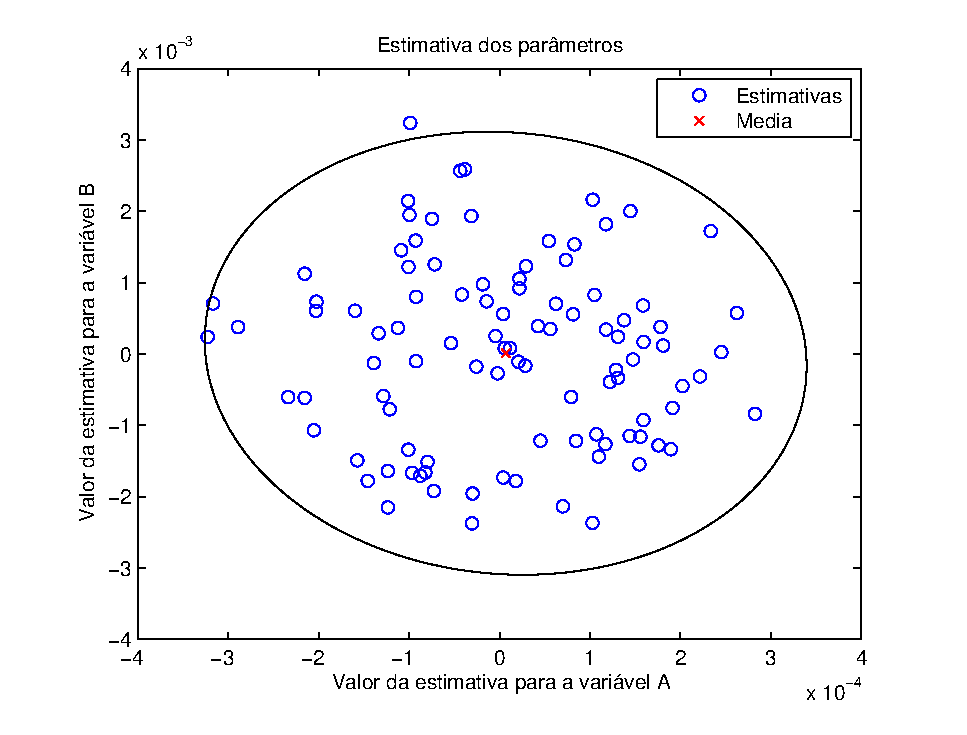
\includegraphics[width=0.95\columnwidth]{figures/si_covar_elipse.eps}
	\caption{Estimativas de um sistema e a elipse representando a regi�o de confian�a para um $\chi$ de 99\%.}
	\label{fig:si_covar_elipse}
\end{figure}
\end{columns}
\end{frame}


%-------------------------------------------------------------------------------------------------
\section{Classes de Modelos}
%-------------------------------------------------------------------------------------------------
\subsection{Classes de modelos lineares} 
%-------------------------------------------------------------------------------------------------
\begin{frame}
\frametitle{Classes de modelos}
\framesubtitle{Sistemas lineares - SISO de tempo discreto}

\begin{columns}
\column{0.6\textwidth}
	\begin{block}{Classe de modelos gen�rica}
	\begin{equation}
		A(z)y(t)=\frac{B(z)}{F(z)}u(t)+\frac{C(z)}{D(z)}e(t)
		\nonumber
	\end{equation}
	\end{block}
	onde:
	\begin{align*}
		A(z, \theta) &= 1+a_1z^{-1}+...+a_{na}z^{-n_a} \\ 
		B(z, \theta) &= b_1z^{-1}+...+b_{nb}z^{-n_b}\\ 
		C(z, \theta) &= 1+c_1z^{-1}+...+c_{nc}z^{-n_c}\\ 
		D(z, \theta) &= 1+d_1z^{-1}+...+d_{nd}z^{-n_d}\\ 
		F(z, \theta) &= 1+f_1z^{-1}+...+f_{nf}z^{-n_f}
	\end{align*}
	
\column{0.4\textwidth}
\begin{small}
\begin{table}
\begin{center}
\label{table:si_modeling_models}
\begin{tabular}{cl}
\hline
        Polin�mios $\neq 1$ & Nome   \\
\hline
        B                 & FIR  	      \\ 
        AB                & ARX           \\ 
        ABC               & ARMAX         \\ 
        AC                & ARMA          \\ 
        ABD               & ARARX         \\ 
        ABCD              & ARARMAX       \\ 
        BF                & OE            \\ 
        BFCD              & Box-Jenkins   \\
\hline
\end{tabular}
\end{center}
\end{table}
\end{small}
\end{columns}
\end{frame}

%-------------------------------------------------------------------------------------------------
\subsection{Classes de modelos n�o lineares} 
%-------------------------------------------------------------------------------------------------
\begin{frame}
\frametitle{Classes de modelos}
\framesubtitle{Sistemas n�o lineares}

\begin{itemize}
  \item Muitos s�o os tipos de classes de modelos para sistemas n�o lineares.
  \item Eles podem ser divididos em dois t�pos principais:
\begin{itemize}
  \item N�o linearidades est�ticas
  \item N�o linearidades din�micas  
\end{itemize}
	\item Diversas classes de modelos se diferenciam pela escolha da base que ir� representar o sistema.
\end{itemize}

\end{frame}

%-------------------------------------------------------------------------------------------------
\begin{frame}
\frametitle{Classes de modelos - Wiener e Hammerstein}
\framesubtitle{Sistemas n�o lineares}

\begin{columns}
\column{0.5\textwidth}
\begin{block}{Representa n�o linearidades est�ticas}
\textcolor{blue}{Wiener}: N�o linearidade acoplada na sa�da do sistema

\textcolor{blue}{Hammerstein}: N�o linearidade acoplada na entrada do sistema
\end{block}

\column{0.5\textwidth}
\begin{figure}[htbp]
\center
\scalebox{0.6} % Change this value to rescale the drawing.
{
\begin{pspicture}(0,-1.6)(9.439062,1.6)
\usefont{T1}{ptm}{m}{n}
\rput(0.52453125,1.31){$u(t)$}
\usefont{T1}{ptm}{m}{n}
\rput(3.9557812,1.31){$f(u(t))$}
\usefont{T1}{ptm}{m}{n}
\rput(7.554531,1.35){$y(t)$}
\usefont{T1}{ptm}{m}{n}
\rput(5.8759375,1.15){Modelo}
\usefont{T1}{ptm}{m}{n}
\rput(5.7834377,0.75){Linear}
\usefont{T1}{ptm}{m}{n}
\rput(2.1957812,1.03){$f(\cdot)$}
\psframe[linewidth=0.04,dimen=outer](3.0,1.6)(1.2,0.4)
\psframe[linewidth=0.04,dimen=outer](6.8,1.6)(5.0,0.4)
\psline[linewidth=0.04cm,arrowsize=0.05291667cm 2.0,arrowlength=1.4,arrowinset=0.4]{->}(3.0,1.0)(5.0,1.0)
\psline[linewidth=0.04cm,arrowsize=0.05291667cm 2.0,arrowlength=1.4,arrowinset=0.4]{->}(0.0,1.0)(1.2,1.0)
\psline[linewidth=0.04cm,arrowsize=0.05291667cm 2.0,arrowlength=1.4,arrowinset=0.4]{->}(6.8,1.0)(8.0,1.0)
\usefont{T1}{ptm}{m}{n}
\rput(0.52453125,-0.69){$u(t)$}
\usefont{T1}{ptm}{m}{n}
\rput(3.9357812,-0.69){$z(t)$}
\usefont{T1}{ptm}{m}{n}
\rput(2.0759375,-0.85){Modelo}
\usefont{T1}{ptm}{m}{n}
\rput(1.9834375,-1.25){Linear}
\usefont{T1}{ptm}{m}{n}
\rput(5.9957814,-0.99){$f(\cdot)$}
\psframe[linewidth=0.04,dimen=outer](3.0,-0.4)(1.2,-1.6)
\psframe[linewidth=0.04,dimen=outer](6.8,-0.4)(5.0,-1.6)
\psline[linewidth=0.04cm,arrowsize=0.05291667cm 2.0,arrowlength=1.4,arrowinset=0.4]{->}(3.0,-1.0)(5.0,-1.0)
\psline[linewidth=0.04cm,arrowsize=0.05291667cm 2.0,arrowlength=1.4,arrowinset=0.4]{->}(0.0,-1.0)(1.2,-1.0)
\psline[linewidth=0.04cm,arrowsize=0.05291667cm 2.0,arrowlength=1.4,arrowinset=0.4]{->}(6.8,-1.0)(8.0,-1.0)
\usefont{T1}{ptm}{m}{n}
\rput(8.204532,-0.65){$y(t)=f(z(t))$}
\end{pspicture} 
}
\caption{Acima: modelo de Hammerstein. Abaixo: Modelo de Wiener.}
\label{fig:nl_models_hammerstein_wiener}
\end{figure}
\end{columns}

\end{frame}
%-------------------------------------------------------------------------------------------------
\begin{frame}
\frametitle{Classes de modelos}
\framesubtitle{Sistemas n�o lineares}

\begin{itemize}
  \item Voltera: Relaciona valores passados da entrada com o valor atual da sa�da.
  	\begin{equation}
		y(t)=\sum_{j=1}^{\infty}\int_{-\infty}^{\infty}\cdots \int_{-\infty}^{\infty}
		h_j(\tau_1, ... ,\tau_j) \prod_{i=1}^{j}u(t-\tau_i)d\tau_i
	\nonumber
	\end{equation}
  \item Redes Neurais: 
  \begin{equation}
	x=f\left ( \sum_{j=1}^{n}\omega_j x_j +b \right )
	\label{eq:nl_models_neural}
  \end{equation}
  \begin{itemize}
    \item Redes neurais multi camadas
    \item Redes neurais recorrente
  \end{itemize}
  \item Fun��es radiais de base: Casos particulares de redes neurais, mas lineares nos parametros $\omega_i$.
  \begin{equation}
	f(y)=\omega_0+\sum_{i}\omega_i \phi (\left \| y-c_i \right \|)
	\label{eq:nl_models_rbf}
  \end{equation}	
\end{itemize}

\end{frame}
%-------------------------------------------------------------------------------------------------
\begin{frame}
\frametitle{Classes de modelos - NARMAX}
\framesubtitle{Sistemas n�o lineares}

\begin{block} {Nonlinear Autoregressive Moving Average model with eXogenous variables}
\begin{equation}
y(t)=\theta^T\Phi_{nl}(y, u, e)
\label{eq:nlin_models_narmax_generic}
\end{equation}
onde $\Phi_{nl}(\cdot)$ denota um campo vetorial que depende dos valores passados de $y(t)$ e presente e passados de
$u(t)$ e $e(t)$; $\theta$ � o vetor de par�metros a ser identificado.
\end{block}

\end{frame}
%-------------------------------------------------------------------------------------------------
\section{Projeto de controladores baseados em dados}
%-------------------------------------------------------------------------------------------------

\begin{frame}
\frametitle{Projeto de controladores baseados em dados}
\framesubtitle{Defini��es}

\begin{block}{Sistema b�sico de controle}
\begin{figure}
\center
% Generated with LaTeXDraw 2.0.8
% Wed Jun 20 23:11:16 BRT 2012
% \usepackage[usenames,dvipsnames]{pstricks}
% \usepackage{epsfig}
% \usepackage{pst-grad} % For gradients
% \usepackage{pst-plot} % For axes
\scalebox{0.7} % Change this value to rescale the drawing.
{
\begin{pspicture}(0,-1.8192188)(9.851875,1.8192188)
\pscircle[linewidth=0.04,dimen=outer](1.431875,-0.79921883){0.2}
\psframe[linewidth=0.04,dimen=outer](4.431875,-0.3992188)(2.631875,-1.1992189)
\psframe[linewidth=0.04,dimen=outer](7.231875,-0.3992188)(5.631875,-1.1992189)
\pscircle[linewidth=0.04,dimen=outer](8.431875,-0.79921883){0.2}
\psline[linewidth=0.04cm,arrowsize=0.05291667cm 2.0,arrowlength=1.4,arrowinset=0.4]{->}(0.031875,-0.79921883)(1.231875,-0.79921883)
\psline[linewidth=0.04cm,arrowsize=0.05291667cm 2.0,arrowlength=1.4,arrowinset=0.4]{->}(1.631875,-0.79921883)(2.631875,-0.79921883)
\psline[linewidth=0.04cm,arrowsize=0.05291667cm 2.0,arrowlength=1.4,arrowinset=0.4]{->}(4.431875,-0.79921883)(5.631875,-0.79921883)
\psline[linewidth=0.04cm,arrowsize=0.05291667cm 2.0,arrowlength=1.4,arrowinset=0.4]{->}(7.231875,-0.79921883)(8.231875,-0.79921883)
\psline[linewidth=0.04cm,arrowsize=0.05291667cm 2.0,arrowlength=1.4,arrowinset=0.4]{->}(8.43,0.39921868)(8.431875,-0.5992188)
\psline[linewidth=0.04cm,arrowsize=0.05291667cm 2.0,arrowlength=1.4,arrowinset=0.4]{->}(8.631875,-0.79921883)(9.831875,-0.79921883)
\psline[linewidth=0.04cm,arrowsize=0.05291667cm 2.0,arrowlength=1.4,arrowinset=0.4]{<-}(1.431875,-0.99921876)(1.431875,-1.7992188)
\psline[linewidth=0.04cm](1.431875,-1.7992188)(9.231875,-1.7992188)
\psline[linewidth=0.04cm](9.231875,-1.7992188)(9.231875,-0.79921883)
\usefont{T1}{ptm}{m}{n}
\rput(1.0698436,-0.48921886){+}
\usefont{T1}{ptm}{m}{n}
\rput(8.069845,-0.48921886){+}
\usefont{T1}{ptm}{m}{n}
\rput(8.069845,-1.0892189){+}
\usefont{T1}{ptm}{m}{n}
\rput(1.6339064,-1.0892189){-}
\usefont{T1}{ptm}{m}{n}
\rput(0.441875,-0.49921885){\small $r(t)$}
\usefont{T1}{ptm}{m}{n}
\rput(3.561875,-0.79921883){\small $C(z, \theta)$}
\usefont{T1}{ptm}{m}{n}
\rput(6.331875,-0.8192189){\small $G_0(z)$}
\usefont{T1}{ptm}{m}{n}
\rput(5.081875,-0.49921885){\small $u(t)$}
\usefont{T1}{ptm}{m}{n}
\rput(1.941875,-0.49921885){\small $\epsilon (t)$}
\usefont{T1}{ptm}{m}{n}
\rput(8.851875,0.12078118){\small $\nu(t)$}
\usefont{T1}{ptm}{m}{n}
\rput(9.271875,-0.49921885){\small $y(t)$}
\psframe[linewidth=0.04,dimen=outer](9.231875,1.2007811)(7.631875,0.40078118)
\usefont{T1}{ptm}{m}{n}
\rput(8.411875,0.7807812){\small $H_0(z)$}
\psline[linewidth=0.04cm](8.43,1.1992186)(8.43,1.7992188)
\usefont{T1}{ptm}{m}{n}
\rput(8.871875,1.5807811){\small $e(t)$}
\end{pspicture} 
}
\caption{Representa��o de um sistema de controle em malha fechada, com ru�do aditivo na sa�da.}
\label{fig:vrft_db_control_loop}
\end{figure}
\end{block}

\begin{equation}
T(z, \theta)=\frac{C(z,\theta)G_0(z)}{1+C(z,\theta)G_0(z)}
\nonumber
\end{equation}

\end{frame}

%-------------------------------------------------------------------------------------------------
%-------------------------------------------------------------------------------------------------

\begin{frame}
\frametitle{Projeto de controladores baseados em dados}
\framesubtitle{Crit�rios de perfomance}

\begin{itemize}
  \item Seguimento de refer�ncia,
  \item Rejei��o ao ru�do e 
  \item Uso reduzido de esfor�o de controle. 
\end{itemize}

Para o objetivo de \textcolor{blue}{seguimento de refer�ncia}, a performance pode ser avaliada pela norma:
\begin{equation}
J_y(\theta)\overset{\underset{\mathrm{\Delta}}{\,}}{=}  \bar{E} \left [ y(t)-y_d(t) \right ]^2 = \bar{E}\left [
(T(z,\theta)-T_d(z))r(t) \right ]^2
\nonumber
\end{equation}

\begin{block}{Controlador ideal - Seguimento de refer�ncia}
\begin{equation}
C_d(z)=\frac{T_d(z)}{G_0(z)(1-T_d(z))}
\nonumber
\end{equation}
\end{block}
\end{frame}

%-------------------------------------------------------------------------------------------------
%-------------------------------------------------------------------------------------------------
%-------------------------------------------------------------------------------------------------
\subsection{Refer�ncia Virtual}
%-------------------------------------------------------------------------------------------------

\begin{frame}
\frametitle{Refer�ncia Virtual para identifica��o de controladores}
\framesubtitle{M�todo VRFT}

\begin{itemize}
  \item M�todo VRFT utiliza refer�ncia virtual para obten��o dos sinais necess�rios � identifica��o. 
\end{itemize}

\begin{figure}
\center
\scalebox{0.7} % Change this value to rescale the drawing.
{
\begin{pspicture}(0,-1.4292188)(9.02,1.4692187)
\pscircle[linewidth=0.04,linestyle=dashed,dash=0.16cm 0.16cm,dimen=outer](1.4,0.97078127){0.2}
\psframe[linewidth=0.04,linestyle=dashed,dash=0.16cm 0.16cm,dimen=outer](4.8,1.3707813)(3.0,0.57078123)
\psframe[linewidth=0.04,dimen=outer](7.6,1.3707813)(6.0,0.57078123)
\psline[linewidth=0.04cm,arrowsize=0.05291667cm 2.0,arrowlength=1.4,arrowinset=0.4]{->}(0.0,0.97078127)(1.2,0.97078127)
\psline[linewidth=0.04cm,linestyle=dashed,dash=0.16cm 0.16cm,arrowsize=0.05291667cm 2.0,arrowlength=1.4,arrowinset=0.4]{->}(1.6,0.97078127)(3.0,0.97078127)
\psline[linewidth=0.04cm,arrowsize=0.05291667cm 2.0,arrowlength=1.4,arrowinset=0.4]{->}(4.8,0.97078127)(6.0,0.97078127)
\psline[linewidth=0.04cm](7.6,0.97078127)(9.0,0.97078127)
\psline[linewidth=0.04cm,linestyle=dashed,dash=0.16cm 0.16cm,arrowsize=0.05291667cm 2.0,arrowlength=1.4,arrowinset=0.4]{<-}(1.4,0.7707813)(1.4,-0.02921875)
\psline[linewidth=0.04cm,linestyle=dashed,dash=0.16cm 0.16cm](1.4,-0.02921875)(8.4,-0.02921875)
\psline[linewidth=0.04cm,linestyle=dashed,dash=0.16cm 0.16cm](8.4,-0.02921875)(8.4,0.97078127)
\usefont{T1}{ptm}{m}{n}
\rput(1.1126562,1.2807813){+}
\usefont{T1}{ptm}{m}{n}
\rput(1.6473438,0.68078125){-}
\usefont{T1}{ptm}{m}{n}
\rput(0.47,1.2707813){\small $\bar{r}(t)$}
\usefont{T1}{ptm}{m}{n}
\rput(3.99,0.97078127){\small $C(z, \theta)$}
\usefont{T1}{ptm}{m}{n}
\rput(6.76,0.9507812){\small $G_0(z)$}
\usefont{T1}{ptm}{m}{n}
\rput(5.51,1.2707813){\small $u(t)$}
\usefont{T1}{ptm}{m}{n}
\rput(2.25,1.2707813){\small $\epsilon (t)$}
\usefont{T1}{ptm}{m}{n}
\rput(8.3,1.2707813){\small $y(t)$}
\psframe[linewidth=0.04,dimen=outer](6.0,-0.62921876)(3.8,-1.4292188)
\usefont{T1}{ptm}{m}{n}
\rput(4.91,-1.0492188){\small $T_d^{-1}(z)$}
\psline[linewidth=0.04cm](9.0,0.97078127)(9.0,-1.0292188)
\psline[linewidth=0.04cm](9.0,-1.0292188)(6.0,-1.0292188)
\psline[linewidth=0.04cm](3.8,-1.0292188)(0.0,-1.0292188)
\psline[linewidth=0.04cm](0.0,-1.0292188)(0.0,0.97078127)
\end{pspicture} 
}
\label{fig:vrft_method_cl}
\end{figure}

\begin{itemize}
  \item O m�todo VRFT faz com que a fun��o custo a ser minimizada seja quadr�tica em $\theta$, n�o recaindo em m�nimos
  locais.
\end{itemize}
\begin{equation}
J_{VR}^N(\theta)=\frac{1}{N}\sum_{t=1}^{N}(u_L(t)-\varphi_L^T(t)\theta)^2
\nonumber
\end{equation}

\begin{equation}
\varphi_L(t)=\beta(z)\epsilon_L(t)
\nonumber
\end{equation}

\end{frame}
%-------------------------------------------------------------------------------------------------
%-------------------------------------------------------------------------------------------------

\begin{frame}
\frametitle{Refer�ncia Virtual para identifica��o de controladores}
\framesubtitle{M�todo VRFT - fun��o custo de um sistem hipot�tico}

\begin{figure}
\center
% Generated with LaTeXDraw 2.0.8
% Mon Jul 02 22:05:15 BRT 2012
% \usepackage[usenames,dvipsnames]{pstricks}
% \usepackage{epsfig}
% \usepackage{pst-grad} % For gradients
% \usepackage{pst-plot} % For axes
\scalebox{0.55} % Change this value to rescale the drawing.
{
\begin{pspicture}(0,-4.62)(11.799063,4.62)
\psbezier[linewidth=0.04](0.9,3.3)(2.1,3.2)(2.0225368,2.3742967)(2.1565964,1.5166456)(2.290656,0.6589943)(2.616248,-1.3127834)(3.008854,-0.5402044)(3.4014597,0.23237456)(3.6584003,0.8693678)(3.811938,0.20167358)(3.9654756,-0.4660206)(4.5199084,-3.4794219)(5.1017394,-3.533306)(5.68357,-3.5871902)(8.0,1.8)(9.5,3.2)
\psbezier[linewidth=0.04,linestyle=dashed,dash=0.16cm 0.16cm](0.4,2.2)(2.2,-2.6)(3.960841,-3.4989967)(5.12,-3.54)(6.279159,-3.5810034)(9.3,-1.9)(10.6,1.9)
\psline[linewidth=0.04cm,arrowsize=0.05291667cm 4.0,arrowlength=1.4,arrowinset=0.4]{<-}(1.1,4.6)(1.2,-4.6)
\psline[linewidth=0.04cm,arrowsize=0.05291667cm 4.0,arrowlength=1.4,arrowinset=0.4]{->}(0.0,-3.9)(11.3,-3.9)
\psline[linewidth=0.04cm,linestyle=dotted,dotsep=0.16cm](5.1,-4.0)(5.0,3.1)
\usefont{T1}{ppl}{m}{n}
\rput(5.114531,-4.19){$\theta^*$}
\usefont{T1}{ppl}{m}{n}
\rput(11.014531,-4.19){$\theta$}
\usefont{T1}{ppl}{m}{n}
\rput(0.5545313,4.01){$J(\theta)$}
\usefont{T1}{ppl}{m}{n}
\rput(2.5545313,2.71){$J_y$}
\usefont{T1}{ppl}{m}{n}
\rput(3.2145312,-1.79){$J_{VR}$}
\end{pspicture} 
}
\caption{O valor $\theta^*$ � o ponto de m�nimo de ambas as fun��es custo, logo, minimizando a fun��o custo
$J_{VR}(\theta)$ � o equivalente a minimizar $J_y(\theta)$ sob condi��es ideais.}
\label{fig:vrft_cost_functions}
\end{figure}

\end{frame}
%-------------------------------------------------------------------------------------------------
\section{Projeto de controladores n�o lineares utilizando refer�ncia virtual} 
%-------------------------------------------------------------------------------------------------
%-------------------------------------------------------------------------------------------------

\begin{frame}
\frametitle{Projeto de controladores n�o lineares baseados em dados}
\framesubtitle{Uni�o do algoritmo de identifica��o de sistemas n�o lineares com refer�ncia virtual}

\begin{block}{Defini��es}
- Deseja-se que o sistema n�o linear, se comporte linearmente em malha fechada: $T_d(z)$

- $\mathcal{C}_d$ � quem proporciona isso.
\end{block}

\begin{figure}
\center
% Generated with LaTeXDraw 2.0.8
% Wed Aug 01 22:46:20 BRT 2012
% \usepackage[usenames,dvipsnames]{pstricks}
% \usepackage{epsfig}
% \usepackage{pst-grad} % For gradients
% \usepackage{pst-plot} % For axes
\scalebox{0.75} % Change this value to rescale the drawing.
{
\begin{pspicture}(0,-1.4292188)(9.601875,1.4692189)
\pscircle[linewidth=0.04,linestyle=dashed,dash=0.16cm 0.16cm,dimen=outer](1.981875,0.97078127){0.2}
\psframe[linewidth=0.04,linestyle=dashed,dash=0.16cm 0.16cm,dimen=outer](5.381875,1.3707813)(3.581875,0.57078123)
\psframe[linewidth=0.04,dimen=outer](8.181875,1.3707813)(6.581875,0.57078123)
\psline[linewidth=0.04cm,arrowsize=0.05291667cm 2.0,arrowlength=1.4,arrowinset=0.4]{->}(0.581875,0.97078127)(1.781875,0.97078127)
\psline[linewidth=0.04cm,linestyle=dashed,dash=0.16cm 0.16cm,arrowsize=0.05291667cm 2.0,arrowlength=1.4,arrowinset=0.4]{->}(2.181875,0.97078127)(3.581875,0.97078127)
\psline[linewidth=0.04cm,arrowsize=0.05291667cm 2.0,arrowlength=1.4,arrowinset=0.4]{->}(5.381875,0.97078127)(6.581875,0.97078127)
\psline[linewidth=0.04cm](8.181875,0.97078127)(9.581875,0.97078127)
\psline[linewidth=0.04cm,linestyle=dashed,dash=0.16cm 0.16cm,arrowsize=0.05291667cm 2.0,arrowlength=1.4,arrowinset=0.4]{<-}(1.981875,0.7707813)(1.981875,-0.02921875)
\psline[linewidth=0.04cm,linestyle=dashed,dash=0.16cm 0.16cm](1.981875,-0.02921875)(8.981875,-0.02921875)
\psline[linewidth=0.04cm,linestyle=dashed,dash=0.16cm 0.16cm](8.981875,-0.02921875)(8.981875,0.97078127)
\usefont{T1}{ptm}{m}{n}
\rput(1.6198437,1.2807813){+}
\usefont{T1}{ptm}{m}{n}
\rput(2.1839063,0.68078125){-}
\usefont{T1}{ptm}{m}{n}
\rput(0.991875,1.2707813){\small $\bar{r}(t)$}
\usefont{T1}{ptm}{m}{n}
\rput(4.451875,0.97078127){\small $\mathcal{C}$}
\usefont{T1}{ptm}{m}{n}
\rput(7.341875,0.9907812){\small $\mathcal{S}$}
\usefont{T1}{ptm}{m}{n}
\rput(6.031875,1.2707813){\small $u(t)$}
\usefont{T1}{ptm}{m}{n}
\rput(2.771875,1.2707813){\small $\epsilon (t)$}
\usefont{T1}{ptm}{m}{n}
\rput(8.821875,1.2707813){\small $y(t)$}
\psframe[linewidth=0.04,dimen=outer](6.581875,-0.62921876)(4.381875,-1.4292188)
\usefont{T1}{ptm}{m}{n}
\rput(5.431875,-1.0492188){\small $T_d^{-1}(z)$}
\psline[linewidth=0.04cm](9.581875,0.97078127)(9.581875,-1.0292188)
\psline[linewidth=0.04cm,arrowsize=0.05291667cm 2.0,arrowlength=1.4,arrowinset=0.4]{->}(9.581875,-1.0292188)(6.581875,-1.0292188)
\psline[linewidth=0.04cm](4.381875,-1.0292188)(0.581875,-1.0292188)
\psline[linewidth=0.04cm](0.581875,-1.0292188)(0.581875,0.97078127)
\end{pspicture} 
}
\label{fig:dbnarmax_method_vr}
\end{figure}

\end{frame}

%-------------------------------------------------------------------------------------------------
%-------------------------------------------------------------------------------------------------
\begin{frame}
\frametitle{Projeto de controladores n�o lineares baseados em dados}
\framesubtitle{Uni�o do algoritmo de identifica��o de sistemas n�o lineares com refer�ncia virtual}

\begin{block}{Objetivo para encontrar o controlador}
\begin{eqnarray}
	&&\min_{\theta} J^{VR}(\theta) \nonumber\\
	&&J^{VR}(\theta) \triangleq \frac{1}{N}\sum_{t=1}^N \left[\left( u(t) - C(\bar{\psi}_C(t),\theta) \right)^2\right].
	\nonumber
\end{eqnarray}
\end{block}
\vspace{\baselineskip}

Classes de modelos exploradas:
\begin{itemize}
  \item N�o linearidades est�ticas: Sistema do tipo Wiener
  \item N�o linearidades din�micas: Sistema racional (NARMAX)
\end{itemize}

\end{frame}

%-------------------------------------------------------------------------------------------------
%-------------------------------------------------------------------------------------------------
\subsection{Sistema do tipo Wiener} 
%-------------------------------------------------------------------------------------------------
%-------------------------------------------------------------------------------------------------
\begin{frame}
\frametitle{Projeto de controladores n�o lineares baseados em dados}
\framesubtitle{Sistema do tipo Wiener - N�o linearidade est�tica na sa�da}

\begin{columns}
\column{0.5\textwidth}
Wiener
% WIENER System
\begin{eqnarray}
z(t) & = & G_0(z) u(t) + H_0 (z) e(t) \nonumber \\
y(t) & = & \phi( z(t)) \nonumber
\end{eqnarray}

\begin{figure}
\center
% Generated with LaTeXDraw 2.0.8
% Tue Sep 04 00:22:08 BRT 2012
% \usepackage[usenames,dvipsnames]{pstricks}
% \usepackage{epsfig}
% \usepackage{pst-grad} % For gradients
% \usepackage{pst-plot} % For axes
\scalebox{0.7} % Change this value to rescale the drawing.
{
\begin{pspicture}(0,-1.0367187)(6.8690624,1.0767188)
\pscircle[linewidth=0.04,dimen=outer](3.17,-0.63671875){0.2}
\psline[linewidth=0.04cm,arrowsize=0.05291667cm 2.0,arrowlength=1.4,arrowinset=0.4]{->}(0.37,-0.63671875)(1.17,-0.63671875)
\psframe[linewidth=0.04,dimen=outer](2.37,-0.23671874)(1.17,-1.0367187)
\psline[linewidth=0.04cm,arrowsize=0.05291667cm 2.0,arrowlength=1.4,arrowinset=0.4]{->}(3.37,-0.63671875)(4.37,-0.63671875)
\psframe[linewidth=0.04,dimen=outer](5.57,-0.23671874)(4.37,-1.0367187)
\psline[linewidth=0.04cm,arrowsize=0.05291667cm 2.0,arrowlength=1.4,arrowinset=0.4]{->}(2.37,-0.63671875)(2.97,-0.63671875)
\psline[linewidth=0.04cm,arrowsize=0.05291667cm 2.0,arrowlength=1.4,arrowinset=0.4]{->}(5.57,-0.63671875)(6.37,-0.63671875)
\usefont{T1}{ppl}{m}{n}
\rput(3.7245312,-0.32671875){$z(t)$}
\usefont{T1}{ppl}{m}{n}
\rput(0.48453125,-0.32671875){$u(t)$}
\usefont{T1}{ppl}{m}{n}
\rput(6.284531,-0.32671875){$y(t)$}
\usefont{T1}{ppl}{m}{n}
\rput(4.934531,-0.62671876){$\phi(\cdot)$}
\usefont{T1}{ppl}{m}{n}
\rput(1.7345313,-0.62671876){$G_0(z)$}
\psline[linewidth=0.04cm,arrowsize=0.05291667cm 2.0,arrowlength=1.4,arrowinset=0.4]{->}(0.37,0.56328124)(1.17,0.56328124)
\psframe[linewidth=0.04,dimen=outer](2.37,0.9632813)(1.17,0.16328125)
\psline[linewidth=0.04cm](2.37,0.56328124)(3.17,0.56328124)
\usefont{T1}{ppl}{m}{n}
\rput(0.48453125,0.87328124){$e(t)$}
\usefont{T1}{ppl}{m}{n}
\rput(1.7345313,0.59328127){$H_0(z)$}
\psline[linewidth=0.04cm,arrowsize=0.05291667cm 2.0,arrowlength=1.4,arrowinset=0.4]{->}(3.17,0.56328124)(3.17,-0.43671876)
\end{pspicture} 
}
\label{fig:Wiener}
\end{figure}

\column{0.5\textwidth}
Controlador: Hammerstein
% HAMMERSTEIN Controller
\begin{eqnarray}
u(t) & = & C_d'(z) v(t)  \nonumber\\
v(t) & = & r(t) - \psi( y(t) )\nonumber
\end{eqnarray}

\begin{figure}[htbp]
\center
% Generated with LaTeXDraw 2.0.8
% Sun Sep 02 10:59:53 BRT 2012
% \usepackage[usenames,dvipsnames]{pstricks}
% \usepackage{epsfig}
% \usepackage{pst-grad} % For gradients
% \usepackage{pst-plot} % For axes
\scalebox{0.7} % Change this value to rescale the drawing.
{
\begin{pspicture}(0,-1.0367187)(4.6990623,1.0767188)
\pscircle[linewidth=0.04,dimen=outer](1.2,0.56328124){0.2}
\psline[linewidth=0.04cm,arrowsize=0.05291667cm 2.0,arrowlength=1.4,arrowinset=0.4]{->}(0.0,0.56328124)(1.0,0.56328124)
\psline[linewidth=0.04cm,arrowsize=0.05291667cm 2.0,arrowlength=1.4,arrowinset=0.4]{->}(1.4,0.56328124)(2.2,0.56328124)
\psframe[linewidth=0.04,dimen=outer](3.4,0.9632813)(2.2,0.16328125)
\psline[linewidth=0.04cm](1.2,-0.63671875)(2.2,-0.63671875)
\psframe[linewidth=0.04,dimen=outer](3.4,-0.23671874)(2.2,-1.0367187)
\psline[linewidth=0.04cm,arrowsize=0.05291667cm 2.0,arrowlength=1.4,arrowinset=0.4]{->}(1.2,-0.63671875)(1.2,0.36328125)
\psline[linewidth=0.04cm,arrowsize=0.05291667cm 2.0,arrowlength=1.4,arrowinset=0.4]{->}(3.4,0.56328124)(4.2,0.56328124)
\psline[linewidth=0.04cm,arrowsize=0.05291667cm 2.0,arrowlength=1.4,arrowinset=0.4]{<-}(3.4,-0.63671875)(4.2,-0.63671875)
\usefont{T1}{ptm}{m}{n}
\rput(0.48453125,0.87328124){$r(t)$}
\usefont{T1}{ptm}{m}{n}
\rput(4.114531,0.87328124){$u(t)$}
\usefont{T1}{ptm}{m}{n}
\rput(4.114531,-0.32671875){$y(t)$}
\usefont{T1}{ptm}{m}{n}
\rput(1.7145313,0.87328124){$v(t)$}
\usefont{T1}{ptm}{m}{n}
\rput(2.7645311,-0.62671876){$\psi(\cdot)$}
\usefont{T1}{ptm}{m}{n}
\rput(2.7745314,0.5732812){$C_d'(z)$}
\psline[linewidth=0.04cm](1.38,0.34328124)(1.54,0.34328124)
\end{pspicture} 
}
\label{fig:dbnarmax_method_vr}
\end{figure}
\end{columns}

%It is clearly seen that even in this standard case the ideal controller is not
%a function of the tracking error $r(t)-y(t)$, but instead a function of $r(t)$ and of $y(t)$ separately.
\begin{block}{Observa��o}
Fica claro que mesmo no caso padr�o o controlador ideal n�o � uma fun��o do erro $r(t)-y(t)$, mas sim de $r(t)$ e
$y(t)$ separadamente.
\end{block}

\end{frame}

%-------------------------------------------------------------------------------------------------
%-------------------------------------------------------------------------------------------------
\begin{frame}
\frametitle{Projeto de controladores n�o lineares baseados em dados}
\framesubtitle{Sistema do tipo Wiener - N�o linearidade est�tica na sa�da}
\fontsize{8}{8}\selectfont
Assumindo que a refer�ncia $r(t)$ seja constante, uma topologia alternativa � tornar o controlador dependente do erro de
refer�ncia.
\begin{block}{Controlador dependente do erro de refer�ncia}
\begin{eqnarray}
u(t) & = & C'(z,\theta) v(t) \nonumber\\
v(t) & = & \psi( r(t) - y(t),\eta )\nonumber
\end{eqnarray}

onde
\begin{equation}
\psi ( r(t) - y(t) ) = \alpha [r(t)-z(t)]
\nonumber
\end{equation}
\end{block}


\begin{figure}[htbp]
\center
% Generated with LaTeXDraw 2.0.8
% Sat Aug 25 13:00:53 BRT 2012
% \usepackage[usenames,dvipsnames]{pstricks}
% \usepackage{epsfig}
% \usepackage{pst-grad} % For gradients
% \usepackage{pst-plot} % For axes
\scalebox{0.62} % Change this value to rescale the drawing.
{
\begin{pspicture}(0,-2.12)(12.480156,2.1)
\psline[linewidth=0.04cm,arrowsize=0.05291667cm 2.0,arrowlength=1.4,arrowinset=0.4]{->}(0.0471875,0.3)(1.0471874,0.3)
\pscircle[linewidth=0.04,dimen=outer](1.2471875,0.3){0.2}
\psline[linewidth=0.04cm,arrowsize=0.05291667cm 2.0,arrowlength=1.4,arrowinset=0.4]{->}(1.4471874,0.3)(2.36,0.3)
\psframe[linewidth=0.04,dimen=outer](3.56,0.7)(2.36,-0.1)
\psline[linewidth=0.04cm,arrowsize=0.05291667cm 2.0,arrowlength=1.4,arrowinset=0.4]{->}(3.56,0.3)(4.36,0.3)
\psframe[linewidth=0.04,dimen=outer](5.56,0.7)(4.36,-0.1)
\psframe[linewidth=0.04,dimen=outer](8.36,0.7)(7.16,-0.1)
\psframe[linewidth=0.04,dimen=outer](10.96,0.7)(9.76,-0.1)
\psline[linewidth=0.04cm,arrowsize=0.05291667cm 2.0,arrowlength=1.4,arrowinset=0.4]{->}(5.447188,0.3)(7.16,0.3)
\psline[linewidth=0.04cm,arrowsize=0.05291667cm 2.0,arrowlength=1.4,arrowinset=0.4]{<-}(1.2471875,0.1)(1.2471875,-2.1)
\psline[linewidth=0.04cm](1.2471875,-2.1)(11.56,-2.1)
\usefont{T1}{ppl}{m}{n}
\rput(0.45453125,0.61){$r(t)$}
\usefont{T1}{ppl}{m}{n}
\rput(1.5807812,0.61){$\epsilon (t)$}
\usefont{T1}{ppl}{m}{n}
\rput(3.930781,0.57){$v(t)$}
\usefont{T1}{ppl}{m}{n}
\rput(6.365625,0.61){$u(t)$}
\usefont{T1}{ppl}{m}{n}
\rput(9.460782,0.61){$z(t)$}
\usefont{T1}{ppl}{m}{n}
\rput(11.895625,0.61){$y(t)$}
\psline[linewidth=0.04cm](1.4671875,0.08)(1.6671875,0.08)
\psframe[linewidth=0.04,linestyle=dashed,dash=0.16cm 0.16cm,dimen=outer](5.96,1.3)(1.96,-0.7)
\psframe[linewidth=0.04,linestyle=dashed,dash=0.16cm 0.16cm,dimen=outer](11.36,2.1)(6.76,-0.7)
\usefont{T1}{ppl}{m}{n}
\rput(3.950781,-0.99){$\mathcal{C}$}
\usefont{T1}{ppl}{m}{n}
\rput(8.870782,-0.99){$\mathcal{S}$}
\usefont{T1}{ppl}{m}{n}
\rput(2.9207811,0.31){$\psi(\cdot)$}
\usefont{T1}{ppl}{m}{n}
\rput(10.320781,0.31){$\phi(\cdot)$}
\usefont{T1}{ppl}{m}{n}
\rput(4.910781,0.31){$C'(z)$}
\usefont{T1}{ppl}{m}{n}
\rput(7.720781,0.31){$G_0(z)$}
\psframe[linewidth=0.04,dimen=outer](8.36,1.7)(7.16,0.9)
\usefont{T1}{ppl}{m}{n}
\rput(7.720781,1.29){$H_0(z)$}
\psline[linewidth=0.04cm](8.36,1.3)(8.96,1.3)
\psline[linewidth=0.04cm,arrowsize=0.05291667cm 2.0,arrowlength=1.4,arrowinset=0.4]{->}(8.96,1.3)(8.96,0.5)
\pscircle[linewidth=0.04,dimen=outer](8.96,0.3){0.2}
\psline[linewidth=0.04cm,arrowsize=0.05291667cm 2.0,arrowlength=1.4,arrowinset=0.4]{->}(8.36,0.3)(8.76,0.3)
\psline[linewidth=0.04cm,arrowsize=0.05291667cm 2.0,arrowlength=1.4,arrowinset=0.4]{->}(9.16,0.3)(9.76,0.3)
\psline[linewidth=0.04cm,arrowsize=0.05291667cm 2.0,arrowlength=1.4,arrowinset=0.4]{->}(6.36,1.3)(7.16,1.3)
\usefont{T1}{ppl}{m}{n}
\rput(6.285625,1.61){$e(t)$}
\psline[linewidth=0.04cm,arrowsize=0.05291667cm 2.0,arrowlength=1.4,arrowinset=0.4]{->}(10.96,0.3)(12.16,0.3)
\psline[linewidth=0.04cm](11.56,-2.1)(11.56,0.3)
\end{pspicture} 
}
\caption{Diagrama de blocos de um sistema n�o linear do tipo Wiener.}
\label{fig:vrft_nl_wiener}
\end{figure}

\end{frame}

%-------------------------------------------------------------------------------------------------
%-------------------------------------------------------------------------------------------------
\begin{frame}
\frametitle{Sistema do tipo Wiener}
\framesubtitle{Exemplo num�rico}

\begin{columns}
\column{0.5\textwidth}
\begin{block}{Sistema Real}
\begin{equation}
G_0(z)=\frac{0.5}{z-0.9}
\nonumber
\end{equation}
\begin{equation}
\phi(z(t))=y(t)=1.5z(t)+0.2z^3(t)
\nonumber
\end{equation}  
\end{block}

\column{0.5\textwidth}
\begin{block}{Comportamento desejado}
\begin{equation}
M(z)=\frac{0.4}{z-0.6}
\nonumber
\end{equation} 
\end{block}
\end{columns}
\vspace{\baselineskip}
Classe de controlador (PI):
\begin{equation}
C(z,\theta) = \theta_1 \frac{1}{z-1} + \theta_2 \frac{z}{z-1}
\nonumber
\end{equation}

e
\begin{equation}
\psi (\epsilon(t))= a_1\epsilon (t) + a_2 \epsilon ^2(t) +a_3 \epsilon ^3(t) +a_4 \epsilon ^4(t)
\nonumber
\end{equation}  
\end{frame}

%-------------------------------------------------------------------------------------------------
%-------------------------------------------------------------------------------------------------
\begin{frame}
\frametitle{Sistema do tipo Wiener}
\framesubtitle{Exemplo num�rico}
\fontsize{8}{8}\selectfont

\begin{columns}
\column{0.6\textwidth}
Parte linear do controlador
\begin{equation}
C_d'(z)= \frac{0.8z-0.72}{z-1}
\label{eq:vrft_nl_wiener_cd}
\end{equation}

\begin{block}{Classe do controlador}
\begin{align}\nonumber
u_f(t) =&  \theta_1 \epsilon (t)+ \theta_2 \epsilon ^2(t)+ \theta_3 \epsilon^3(t)+ \theta_4 \epsilon^4(t)+\\ \nonumber
& \theta_6 \epsilon^2(t-1)+  \theta_7 \epsilon^3(t-1)+ \\ & \theta_8 \epsilon^4(t-1)
\label{eq:dbnarmax_ex_wiener_controller}
\end{align}
\end{block}



\column{0.4\textwidth}
100 Monte Carlo experimentos foram realizados e a m�dia das estimativas obtidas foi:

\begin{equation}
\theta_{\text{m�dia}} =\begin{bmatrix}
0.44717 \\ 2.0216\times10^{-3} \\ -6.5181\times10^{-4} \\ -1.608\times10^{-5} \\ -0.40435 \\ -1.6163\times10^{-3} \\
6.1265\times10^{-4}\\ 1.469\times10^{-5} 
\end{bmatrix}
\nonumber
\end{equation}

\end{columns}
\vspace{\baselineskip}

O custo obtido foi: $J^{MR}(\theta_{\text{m�dia}})=3.0078\times10^{-3}$;
\end{frame}

%-------------------------------------------------------------------------------------------------
%-------------------------------------------------------------------------------------------------
% TODO: preciso trocar o \omega por z(t).
\begin{frame}
\frametitle{Sistema do tipo Wiener}
\framesubtitle{Exemplo num�rico}
\fontsize{8}{8}\selectfont

\begin{figure}[htbp] 
	\center 
	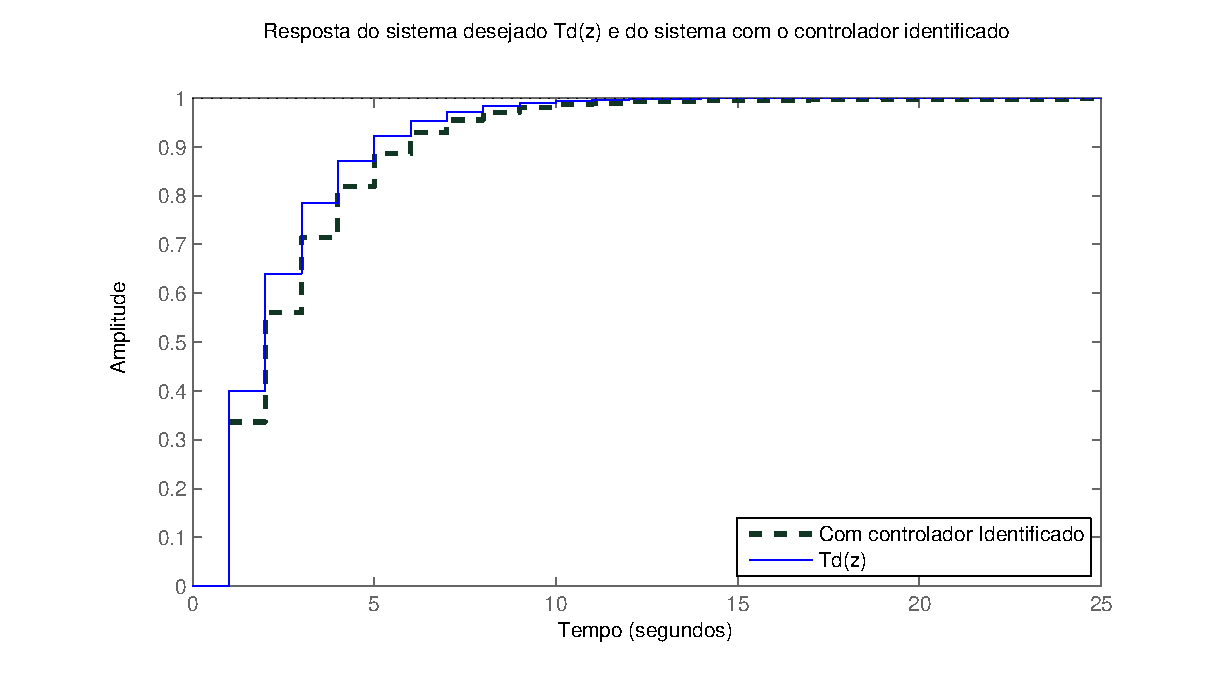
\includegraphics[width=0.95\columnwidth]{figures/vrft_nl_wiener_step.eps}
	\caption{Comparativo da resposta a um degrau unit�rio do modelo de refer�ncia $T_d(z)$ com o sistema real quando o
	controlador controlador n�o linear representado por um modelo NARMAX polinomial � inserido na planta.}
	\label{fig:vrft_nl_wiener_step}
\end{figure}
\end{frame}

%-------------------------------------------------------------------------------------------------
%-------------------------------------------------------------------------------------------------

\begin{frame}
\frametitle{Sistema do tipo Wiener}
\framesubtitle{Exemplo num�rico}
\fontsize{8}{8}\selectfont

\begin{figure}[htbp] 
	\center 
	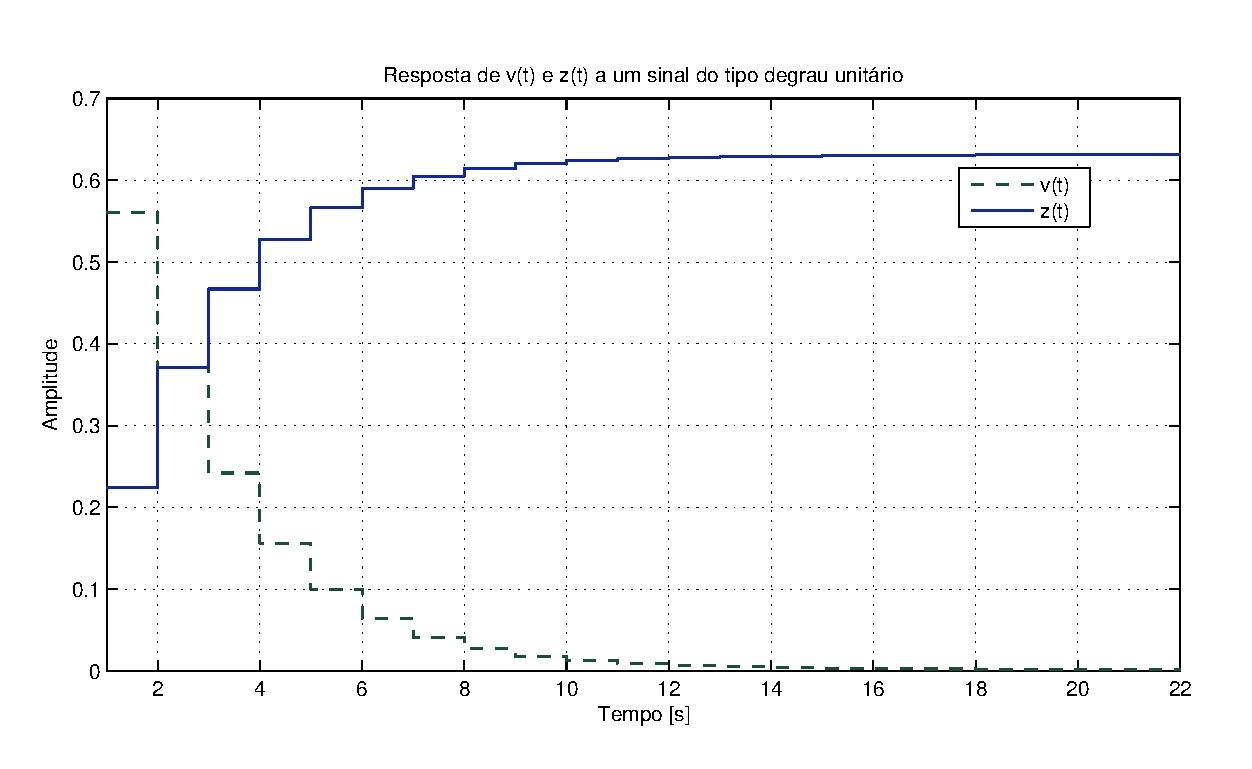
\includegraphics[width=0.9\columnwidth]{figures/vrft_nl_wiener_vz_step.eps}
	\caption{Sinais $v(t)$ e $z(t)$ do sistema apresentado na Figura \ref{fig:vrft_nl_wiener} quando este �
	excitado por um degrau unit�rio.}
	\label{fig:vrft_nl_wiener_vw_step}
\end{figure}

\end{frame}

%-------------------------------------------------------------------------------------------------
%-------------------------------------------------------------------------------------------------
\begin{frame}
\frametitle{Sistema do tipo Wiener}
\framesubtitle{Exemplo num�rico}
\fontsize{8}{8}\selectfont

\begin{figure}[htbp] 
	\center 
	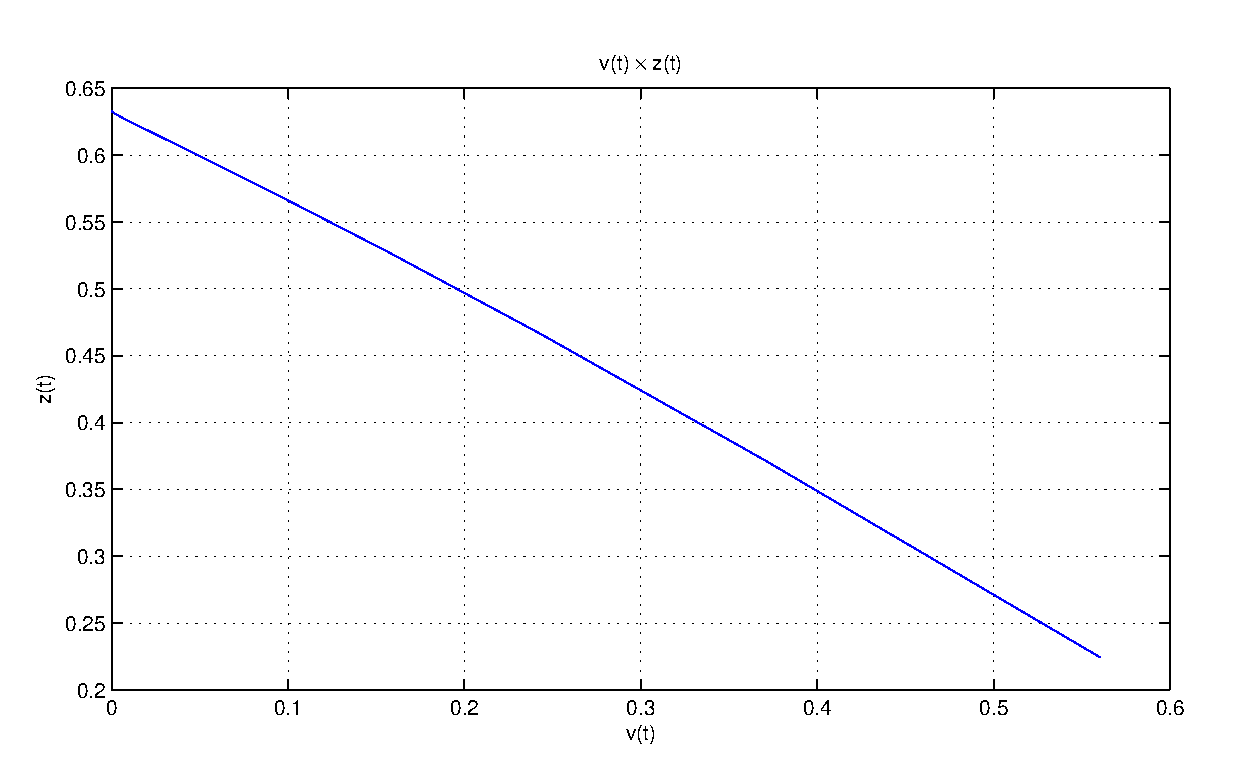
\includegraphics[width=0.9\columnwidth]{figures/vrft_nl_wiener_vz.eps}
	\caption{rela��o entre os sinais $v(t)$ e $z(t)$ quando o sistema � alimentado por um degrau unit�rio}
	\label{fig:vrft_nl_wiener_vw}
\end{figure}

\end{frame}

%-------------------------------------------------------------------------------------------------
%-------------------------------------------------------------------------------------------------
\subsection{Sistemas Racionais} 
%-------------------------------------------------------------------------------------------------
%-------------------------------------------------------------------------------------------------
\begin{frame}
\frametitle{Projeto de controladores n�o lineares baseados em dados}
\framesubtitle{Sistema Racionais - N�o linearidade na din�mica do sistema}

Sistemas racionais
\end{frame}
%-------------------------------------------------------------------------------------------------
%-------------------------------------------------------------------------------------------------
\begin{frame}
\frametitle{Projeto de controladores n�o lineares baseados em dados}
\framesubtitle{Sistema Racionais - N�o linearidade na din�mica do sistema}
\fontsize{7}{7}\selectfont

\begin{block}{}
  Quando a planta � um sistema racional e o comportamento em malha fechada � linear, o controlador �timo pode ser
  tamb�m reprentado por um modelo racional.
\end{block}
\vspace{\baselineskip}

Exemplificando:

\begin{columns}
\column{0.5\textwidth}
\begin{block}{Sistema real}
\begin{equation}
y(t)=\frac{0.5u(t-1)y(t-1)+u(t-1)}{1+0.25y^2(t-2)}
\nonumber
\end{equation}
\end{block}

\column{0.5\textwidth}
Comportamento em malha fechada esperado:
\begin{equation}
T_d(z)=\frac{0.4}{z-0.6}
\nonumber
\end{equation}

\begin{block}{}
\begin{equation}
y(t)=0.4r(t-1)+0.6y(t-1)
\nonumber
\end{equation}
\end{block}

\end{columns}
\vspace{\baselineskip}

\begin{block}{Controlador �timo para este conjunto}
\begin{equation}
u(t)=\frac{0.4r(t)+0.6y(t)+0.1y^2(t-1)r(t)+0.15y(t)y^2(t-1)}{1+0.5y(t)}
\nonumber
\end{equation}
\end{block}

\end{frame}

%-------------------------------------------------------------------------------------------------
%-------------------------------------------------------------------------------------------------
\begin{frame}
\frametitle{Sistema Racionais - N�o linearidade na din�mica do sistema}
\framesubtitle{Exemplo num�rico: $\mathcal{C}_d \in \mathcal{C}$}
\fontsize{7}{7}\selectfont

\begin{block}{Classe de modelos do controlador: $\mathcal{C}_d \in \mathcal{C}$}
\begin{equation}
u(t)=\frac{\theta_1 r(t)+ \theta_2 y(t)+ \theta_3 y^2(t-1)r(t)+ \theta_4 y(t)y^2(t-1)}{1+ \theta_5 y(t)}
\nonumber
\end{equation}
\end{block}
%\vspace{\baselineskip}

Utilizando um sinal PRBS de 254 pontos (ordem 7) e fazendo 100 experimentos de Monte Carlo com um ru�do de vari�ncia de
$\sigma_e^2 = 0.005$
\begin{columns}
\column{0.55\textwidth}
\textcolor{blue}{
\begin{equation}
\theta_{\text{m�dia}}=\begin{bmatrix}
0.4000 & 0.5999 & 0.1001 & 0.1501 & 0.5000
\end{bmatrix}
\nonumber
\end{equation}}
\column{0.45\textwidth}
Custo obtido foi \textcolor{red}{$J_{y}(\theta_{\text{m�dio}})=0.0033$ } e 
\textcolor{red}{$J_{VR}(\theta_{\text{m�dio}})=2.7291\times10{-8}$}
\end{columns}

\begin{columns}
\column{0.6\textwidth}
\begin{figure} 
	\center 
	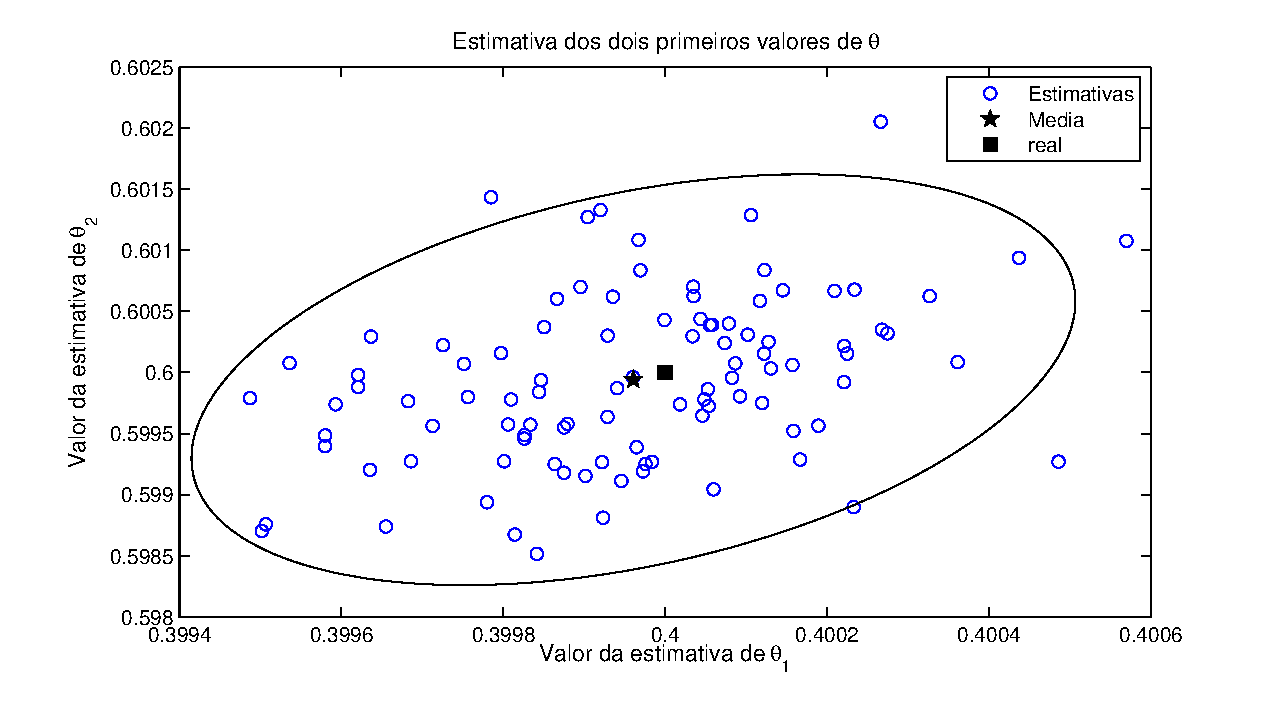
\includegraphics[width=0.99\columnwidth]{figures/vrft_nl_dynamic_t1_t2.eps}
	\label{fig:vrft_nl_dynamic_t1_t2}
\end{figure}

\column{0.5\textwidth}
Erro entre a resposta esperada e a obtida:
\begin{figure} 
	\center 
	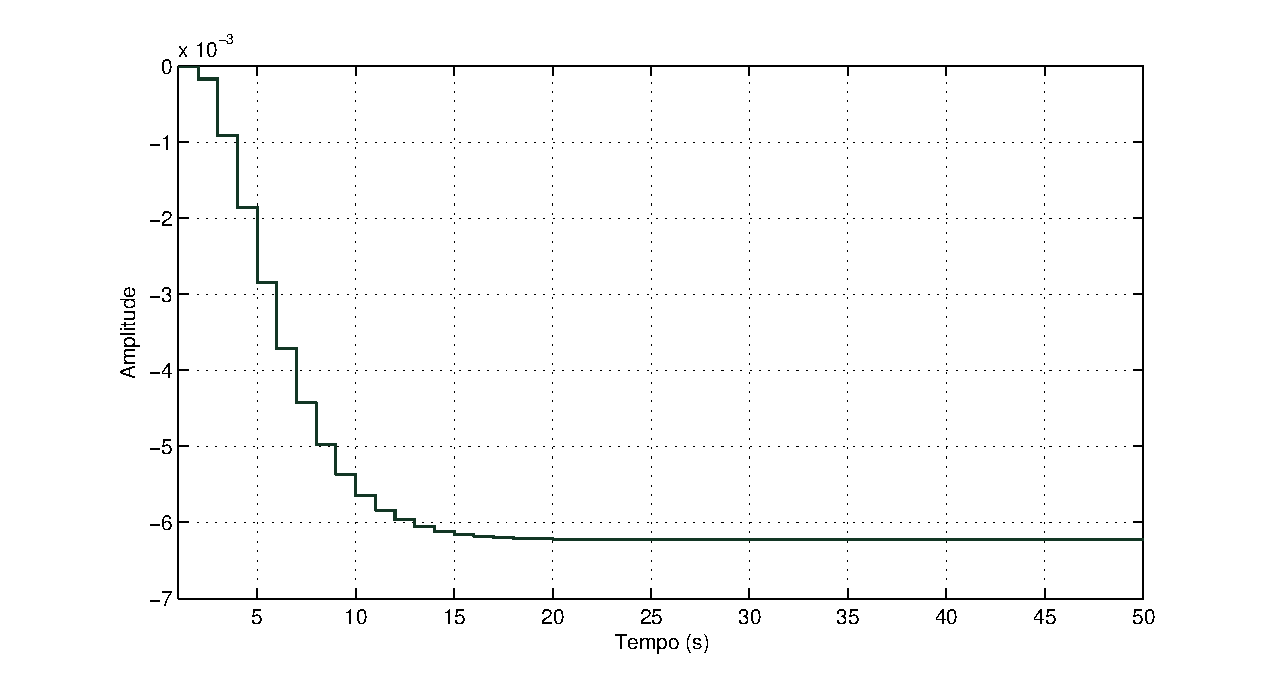
\includegraphics[width=0.99\columnwidth]{figures/vrft_nl_dynamic_erro_step.eps}
	%\caption{Erro entre a resposta esperada e a obtida}
	\label{fig:vrft_nl_dynamic_step_erro}
\end{figure}

\end{columns}
\end{frame}

%-------------------------------------------------------------------------------------------------
%-------------------------------------------------------------------------------------------------
\begin{frame}
\frametitle{Sistema Racionais - N�o linearidade na din�mica do sistema}
\framesubtitle{Exemplo num�rico: $\mathcal{C}_d \notin \mathcal{C}$}
%\fontsize{7}{7}\selectfont

Considerando o mesmo sistema real apresentado anteriormente:
\begin{block}{Classe de modelos do controlador: $\mathcal{C}_d \notin \mathcal{C}$}
\begin{equation}
%u(t)=\frac{\theta_1 r(t)+ \theta_2 y(t)+ \theta_3 y^2(t-1)r(t)+ \theta_4 y(t)y^2(t-1)}{1+ \theta_5 y(t)}
u(t)=\frac{\theta_1 r(t)+ \theta_2 y(t)+ \theta_3 r(t)y(t-1)+ \theta_4 y(t-1)y(t)}{1+ \theta_5 y(t)}
\nonumber
\end{equation}
\end{block}
\vspace{\baselineskip}

Utilizando um sinal PRBS de 254 pontos (ordem 7) e fazendo 100 experimentos de Monte Carlo com um ru�do de vari�ncia de
$\sigma_e^2 = 0.005$

\textcolor{blue}{
\begin{equation}
\theta_{\text{m�dia}}=\begin{bmatrix}
0.4696 & 0.7011 & 0.0083 & 0.0063 & 0.5013
\end{bmatrix}
\nonumber
\end{equation}}

Custo obtido foi 
\textcolor{red}{$J_{y}(\theta_{\text{m�dio}})=1.0999$}

\end{frame}

%-------------------------------------------------------------------------------------------------
%-------------------------------------------------------------------------------------------------
\begin{frame}
\frametitle{Sistema Racionais - N�o linearidade na din�mica do sistema}
\framesubtitle{Exemplo num�rico: $\mathcal{C}_d \notin \mathcal{C}$}

\begin{figure}[htbp] 
	\center 
	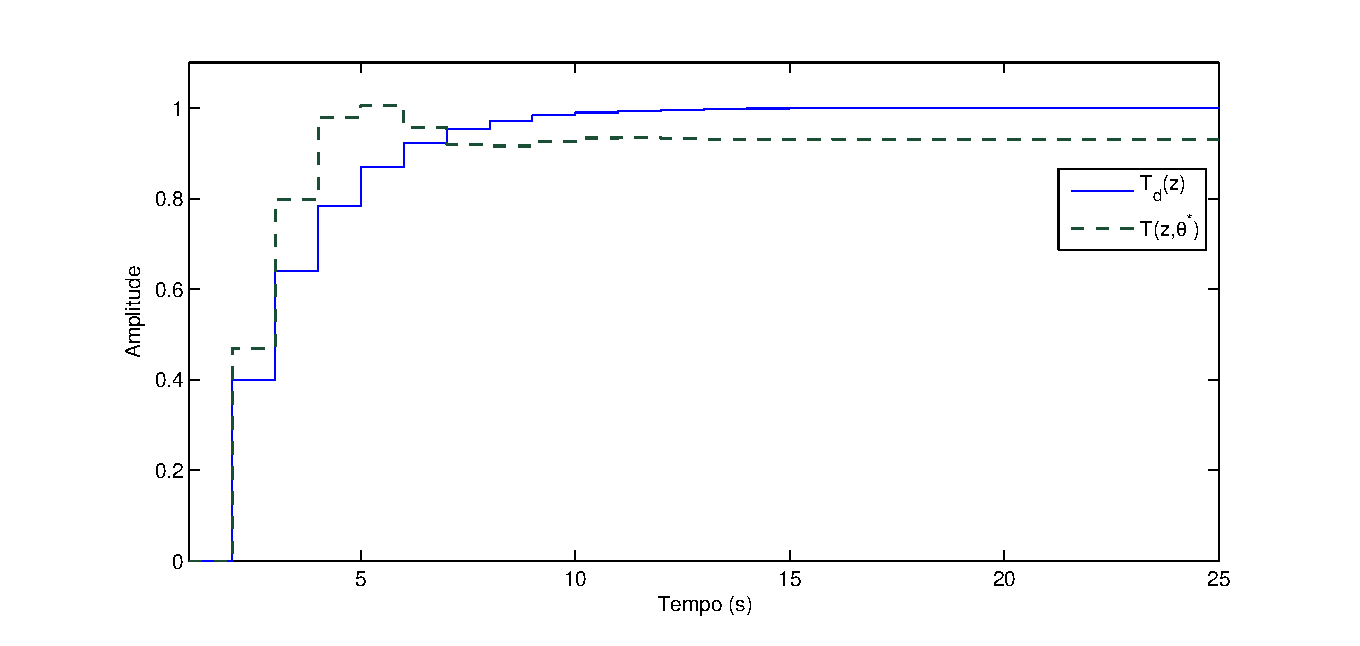
\includegraphics[width=0.95\columnwidth]{figures/vr_rational_notinclass_ex3_step.eps}
	\caption{Exemplo onde $\mathcal{C}_d \notin \mathcal{C}$: Resposta do sistema ao degrau unit�rio para o
	sistema desejado $T_d(z)$ e o sistema quando o controlador parametrizado por $\theta_{\text{m�dio}}$}
	\label{fig:vr_rational_notinclass_ex3_step}
\end{figure}
\end{frame}

%-------------------------------------------------------------------------------------------------
%-------------------------------------------------------------------------------------------------

%-------------------------------------------------------------------------------------------------
\section{Conclus�es} 
%-------------------------------------------------------------------------------------------------

\begin{frame}
\frametitle{Conclus�es}

\begin{itemize}
	\item Utiliza��o de algoritmos de identifica��o de sistemas n�o lineares pode ser estendida para a identifica��o de
	controladores n�o lineares.
	\item Refer�ncia virtual traz diversas vantagens para a obten��o dos dados para alimenta��o dos algoritmos n�o
	lineares.
	\item Resultados obtidos com os exemplos apresentados podem ser considerados satisfat�rios para um grande n�mero de
	aplica��es.
\end{itemize}
\end{frame}

%-------------------------------------------------------------------------------------------------
%-------------------------------------------------------------------------------------------------

\begin{frame}
	\frametitle{Quest�es}
			\linespread{1.3}
\centerline{Muito Obrigado}
\end{frame}

%-------------------------------------------------------------------------------------------------
%-------------------------------------------------------------------------------------------------
% Slides extras
%-------------------------------------------------------------------------------------------------
%\subsection{Sinais utilizados} 
%-------------------------------------------------------------------------------------------------
\begin{frame}
\frametitle{Defini��es}
\framesubtitle{Sinal PRBS}
 
\begin{block}{Sinal PRBS}
\begin{equation}
u(t)=rem(A(z)u(t), 2)=rem(a_1 u(t-1)+...+a_n u(t-n), 2)
\nonumber
\end{equation}
\end{block}

\begin{columns}
\column{0.35\textwidth}

\begin{table}
\fontsize{6}{8}\selectfont
\begin{center}
\begin{tabular}{ccc}
\hline
        Ordem $n$ & $M=2^n-1$ & $a_k$ n�o   \\
        & & zeros para $k$ \\
\hline
        2       & 3        & 1, 2       \\
        3       & 7        & 2, 3       \\
        4       & 15       & 1, 4       \\
        5       & 31       & 2, 5       \\
        6       & 63       & 1, 6       \\
        7       & 127      & 3, 7       \\
        8       & 255      & 1, 2, 7, 8 \\
        9       & 511      & 4, 9       \\
        10      & 1023     & 7, 10      \\
        11      & 2047     & 9, 11      \\
\hline
\end{tabular}
\end{center}
\end{table}

\column{0.7\textwidth}
\begin{figure}[htbp]
	\center
	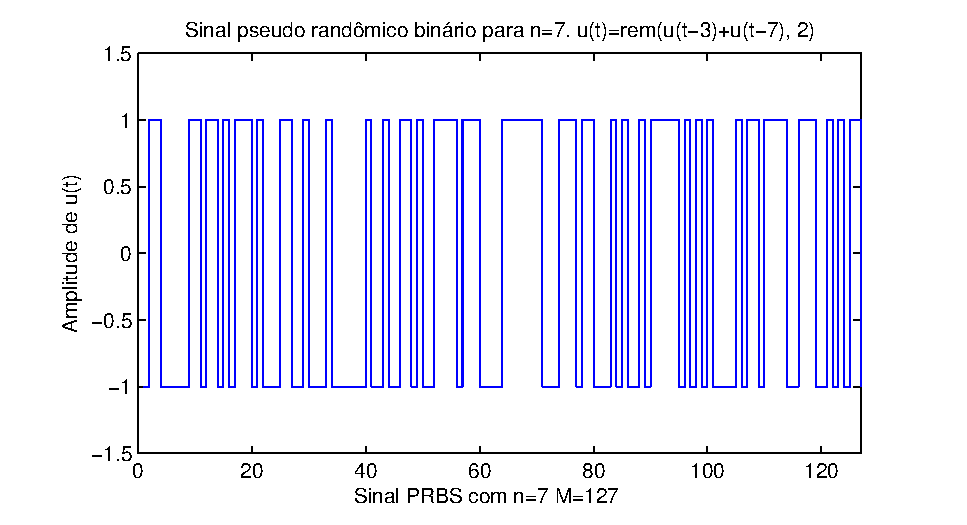
\includegraphics[width=0.95\columnwidth]{figures/si_project_prbs.eps}
	\caption{Sinal PRBS para $n=7$}
	\label{fig:si_project_prbs}
\end{figure}
\end{columns}
\end{frame}



\begin{frame}
	\frametitle{Quest�es}
			\linespread{1.3}
Muito Obrigado.
\end{frame}
\end{document}
